% Created by tikzDevice version 0.12 on 2019-04-24 20:42:01
% !TEX encoding = UTF-8 Unicode
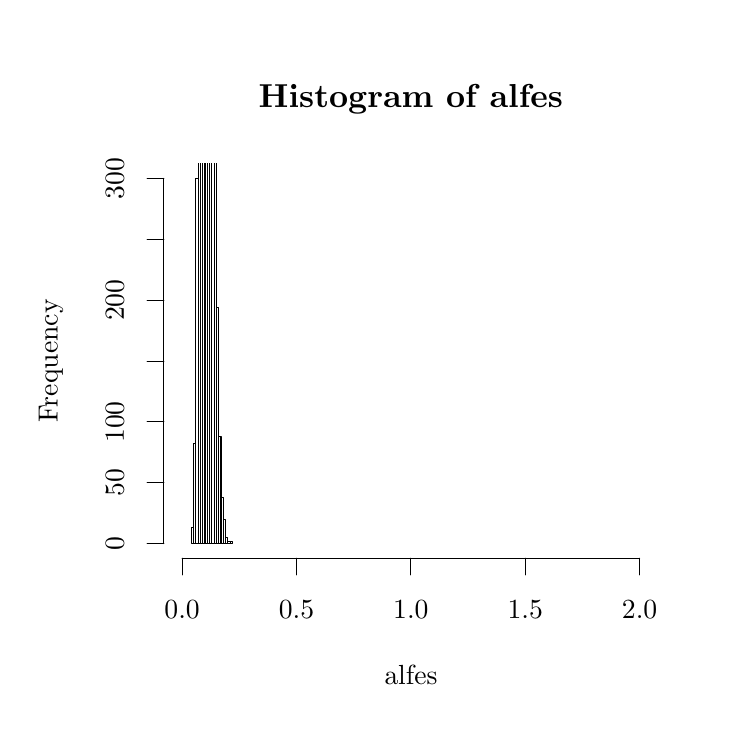
\begin{tikzpicture}[x=1pt,y=1pt]
\definecolor{fillColor}{RGB}{255,255,255}
\path[use as bounding box,fill=fillColor,fill opacity=0.00] (0,0) rectangle (252.94,252.94);
\begin{scope}
\path[clip] (  0.00,  0.00) rectangle (252.94,252.94);
\definecolor{drawColor}{RGB}{0,0,0}

\node[text=drawColor,anchor=base,inner sep=0pt, outer sep=0pt, scale=  1.20] at (138.47,224.20) {\bfseries Histogram of alfes};

\node[text=drawColor,anchor=base,inner sep=0pt, outer sep=0pt, scale=  1.00] at (138.47, 15.60) {alfes};

\node[text=drawColor,rotate= 90.00,anchor=base,inner sep=0pt, outer sep=0pt, scale=  1.00] at ( 10.80,132.47) {Frequency};
\end{scope}
\begin{scope}
\path[clip] (  0.00,  0.00) rectangle (252.94,252.94);
\definecolor{drawColor}{RGB}{0,0,0}

\path[draw=drawColor,line width= 0.4pt,line join=round,line cap=round] ( 55.81, 61.20) -- (221.13, 61.20);

\path[draw=drawColor,line width= 0.4pt,line join=round,line cap=round] ( 55.81, 61.20) -- ( 55.81, 55.20);

\path[draw=drawColor,line width= 0.4pt,line join=round,line cap=round] ( 97.14, 61.20) -- ( 97.14, 55.20);

\path[draw=drawColor,line width= 0.4pt,line join=round,line cap=round] (138.47, 61.20) -- (138.47, 55.20);

\path[draw=drawColor,line width= 0.4pt,line join=round,line cap=round] (179.80, 61.20) -- (179.80, 55.20);

\path[draw=drawColor,line width= 0.4pt,line join=round,line cap=round] (221.13, 61.20) -- (221.13, 55.20);

\node[text=drawColor,anchor=base,inner sep=0pt, outer sep=0pt, scale=  1.00] at ( 55.81, 39.60) {0.0};

\node[text=drawColor,anchor=base,inner sep=0pt, outer sep=0pt, scale=  1.00] at ( 97.14, 39.60) {0.5};

\node[text=drawColor,anchor=base,inner sep=0pt, outer sep=0pt, scale=  1.00] at (138.47, 39.60) {1.0};

\node[text=drawColor,anchor=base,inner sep=0pt, outer sep=0pt, scale=  1.00] at (179.80, 39.60) {1.5};

\node[text=drawColor,anchor=base,inner sep=0pt, outer sep=0pt, scale=  1.00] at (221.13, 39.60) {2.0};

\path[draw=drawColor,line width= 0.4pt,line join=round,line cap=round] ( 49.20, 66.48) -- ( 49.20,198.47);

\path[draw=drawColor,line width= 0.4pt,line join=round,line cap=round] ( 49.20, 66.48) -- ( 43.20, 66.48);

\path[draw=drawColor,line width= 0.4pt,line join=round,line cap=round] ( 49.20, 88.48) -- ( 43.20, 88.48);

\path[draw=drawColor,line width= 0.4pt,line join=round,line cap=round] ( 49.20,110.47) -- ( 43.20,110.47);

\path[draw=drawColor,line width= 0.4pt,line join=round,line cap=round] ( 49.20,132.47) -- ( 43.20,132.47);

\path[draw=drawColor,line width= 0.4pt,line join=round,line cap=round] ( 49.20,154.47) -- ( 43.20,154.47);

\path[draw=drawColor,line width= 0.4pt,line join=round,line cap=round] ( 49.20,176.47) -- ( 43.20,176.47);

\path[draw=drawColor,line width= 0.4pt,line join=round,line cap=round] ( 49.20,198.47) -- ( 43.20,198.47);

\node[text=drawColor,rotate= 90.00,anchor=base,inner sep=0pt, outer sep=0pt, scale=  1.00] at ( 34.80, 66.48) {0};

\node[text=drawColor,rotate= 90.00,anchor=base,inner sep=0pt, outer sep=0pt, scale=  1.00] at ( 34.80, 88.48) {50};

\node[text=drawColor,rotate= 90.00,anchor=base,inner sep=0pt, outer sep=0pt, scale=  1.00] at ( 34.80,110.47) {100};

\node[text=drawColor,rotate= 90.00,anchor=base,inner sep=0pt, outer sep=0pt, scale=  1.00] at ( 34.80,154.47) {200};

\node[text=drawColor,rotate= 90.00,anchor=base,inner sep=0pt, outer sep=0pt, scale=  1.00] at ( 34.80,198.47) {300};
\end{scope}
\begin{scope}
\path[clip] ( 49.20, 61.20) rectangle (227.75,203.75);
\definecolor{drawColor}{RGB}{0,0,0}

\path[draw=drawColor,line width= 0.4pt,line join=round,line cap=round] ( 59.12, 66.48) rectangle ( 59.95, 72.20);

\path[draw=drawColor,line width= 0.4pt,line join=round,line cap=round] ( 59.95, 66.48) rectangle ( 60.77,102.56);

\path[draw=drawColor,line width= 0.4pt,line join=round,line cap=round] ( 60.77, 66.48) rectangle ( 61.60,198.47);

\path[draw=drawColor,line width= 0.4pt,line join=round,line cap=round] ( 61.60, 66.48) rectangle ( 62.43,414.92);

\path[draw=drawColor,line width= 0.4pt,line join=round,line cap=round] ( 62.43, 66.48) rectangle ( 63.25,674.50);

\path[draw=drawColor,line width= 0.4pt,line join=round,line cap=round] ( 63.25, 66.48) rectangle ( 64.08,821.00);

\path[draw=drawColor,line width= 0.4pt,line join=round,line cap=round] ( 64.08, 66.48) rectangle ( 64.91,870.27);

\path[draw=drawColor,line width= 0.4pt,line join=round,line cap=round] ( 64.91, 66.48) rectangle ( 65.73,718.93);

\path[draw=drawColor,line width= 0.4pt,line join=round,line cap=round] ( 65.73, 66.48) rectangle ( 66.56,528.43);

\path[draw=drawColor,line width= 0.4pt,line join=round,line cap=round] ( 66.56, 66.48) rectangle ( 67.39,349.81);

\path[draw=drawColor,line width= 0.4pt,line join=round,line cap=round] ( 67.39, 66.48) rectangle ( 68.21,226.18);

\path[draw=drawColor,line width= 0.4pt,line join=round,line cap=round] ( 68.21, 66.48) rectangle ( 69.04,151.83);

\path[draw=drawColor,line width= 0.4pt,line join=round,line cap=round] ( 69.04, 66.48) rectangle ( 69.86,105.20);

\path[draw=drawColor,line width= 0.4pt,line join=round,line cap=round] ( 69.86, 66.48) rectangle ( 70.69, 83.20);

\path[draw=drawColor,line width= 0.4pt,line join=round,line cap=round] ( 70.69, 66.48) rectangle ( 71.52, 75.28);

\path[draw=drawColor,line width= 0.4pt,line join=round,line cap=round] ( 71.52, 66.48) rectangle ( 72.34, 68.68);

\path[draw=drawColor,line width= 0.4pt,line join=round,line cap=round] ( 72.34, 66.48) rectangle ( 73.17, 67.36);

\path[draw=drawColor,line width= 0.4pt,line join=round,line cap=round] ( 73.17, 66.48) rectangle ( 74.00, 67.36);
\end{scope}
\end{tikzpicture}
\begin{tikzpicture}[x=1pt,y=1pt]
\definecolor{fillColor}{RGB}{255,255,255}
\path[use as bounding box,fill=fillColor,fill opacity=0.00] (0,0) rectangle (252.94,252.94);
\begin{scope}
\path[clip] (  0.00,  0.00) rectangle (252.94,252.94);
\definecolor{drawColor}{RGB}{0,0,0}

\node[text=drawColor,anchor=base,inner sep=0pt, outer sep=0pt, scale=  1.20] at (138.47,224.20) {\bfseries Histogram of alfes};
\end{scope}
\end{tikzpicture}
\begin{tikzpicture}[x=1pt,y=1pt]
\definecolor{fillColor}{RGB}{255,255,255}
\path[use as bounding box,fill=fillColor,fill opacity=0.00] (0,0) rectangle (252.94,252.94);
\begin{scope}
\path[clip] (  0.00,  0.00) rectangle (252.94,252.94);
\definecolor{drawColor}{RGB}{0,0,0}

\node[text=drawColor,anchor=base,inner sep=0pt, outer sep=0pt, scale=  1.20] at (138.47,224.20) {\bfseries Histogram of alfes};
\end{scope}
\end{tikzpicture}
